% !TeX root = ../main.tex

\chapter{系统实现}
\label{chap:impl}

如\autoref{chap:design}所述,本系统主要由三部分组成:控制器、客户端和存储单元。
他们的实现基于开源的Storage Performence Development Kit (SPDK)~\cite{yang2017spdk}工具和用于网络访问NVMe设备的NVMe-oF~\cite{nvmeof2016}等技术。

\section{控制器}
\label{sec:impl-controller}

本系统的控制器是用C++实现的,代码共计418行,其职责是根据用户的请求,为其分配存储单元,并管理存储单元。
控制器通过RPC与客户端库和存储单元通信。
在本系统中,用户和存储单元的SLA曲线被采样后存放在数组中,SLA曲线的加、减等运算都在控制器中通过数组操作实现。
控制器存放着所有数据块的占有状态及从用户的地址空间到存储单元的地址空间的映射。
当需要启用新的存储单元时,控制器通过RPC告知存储服务器上的\JF{加内容}。

由于客户端库直接通过网络访问存储单元,所以为了数据的安全性,需要加入访问控制。
本系统在新租户加入系统时,由控制器生成token同时发送给租户和分配给它的存储单元。
只有当存储单元收到正确的token时,才允许用户进行访问。
在网络传输的过程中,数据被加密,以免数据泄露。

\section{客户端}
\label{sec:impl-client}

本系统的客户端IO调度器是利用SPDK实现的,C代码共计455行。
该部分的主要功能是保证各个租户都处在其自身的SLA曲线中,从而使得各个存储单元整体运行在各自的SLA曲线下,得到稳定的尾延迟。
IO调度器的实现基于quota,在各个时间片中,每个租户都被记录下发送的读写吞吐。
如\autoref{chap:design}所述,当租户发送读请求时,IO调度器根据SLA曲线查询当前写吞吐对应的最大读吞吐,并依据其对读请求进行限速;
当租户发送写请求时,IO调度器根据SLA曲线查询发送该写请求后当前读吞吐是否将超过了新的写吞吐对应的最大读吞吐,并据此对写请求进行限速。

\section{存储单元}
\label{sec:impl-storage-unit}

本系统存储单元部分的软件代码是在SPDK实现了一个新的bdev层,对SPDK的代码增删共计1699行。
为了保证系统的低延迟,本系统的存储单元利用SPDK的用户态NVMe驱动进行SSD访问。
SPDK通过绑定CPU核进行轮询,并直接将NVMe队列映射到用户内存空间的方式提高访问效率。
在我们的实验中,1个CPU核就可以跑满Samsung PM963的带宽。
目前的实现利用存储服务器上的DRAM作为写请求的缓冲区。
在SSD的读窗口中,对它的写请求数据直接被存入存储服务器上预先开辟的内存池中。
为了避免读窗口阻塞租户的写队列,存储服务器直接向租户返回写成功的信号。

\begin{figure}[h]
  \centering
  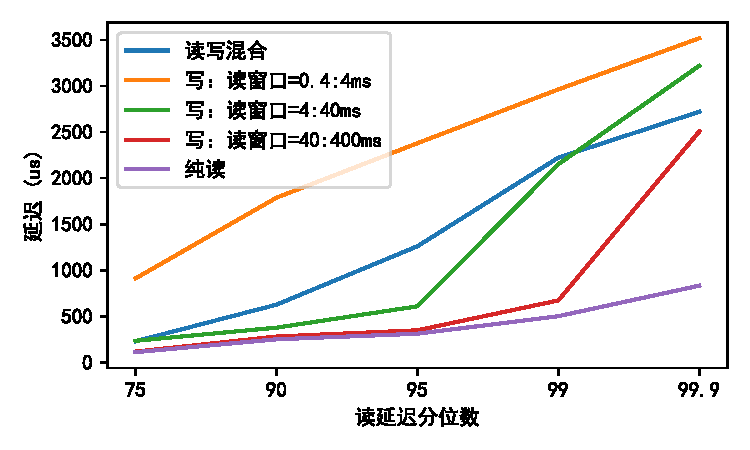
\includegraphics[width=0.7\textwidth]{thesis-window-size.pdf}
  \caption{
        窗口大小的选择。
      }
  \label{fig:impl-window-size}
\end{figure}

\autoref{chap:design}提到,读窗口和写窗口的时长不能被选择得过小,否则过多的窗口切换会影响尾延迟。
\JF{加图}具体描述了同一比例下,不同读写窗口大小对尾延迟的改善程度。
如图所示,当读写窗口的总长度为数十毫秒时,相当于每秒切换窗口数十次,95\%的尾延迟与无读写干扰时相近;
当读写窗口的总长度为数百毫秒时,相当于每秒切换窗口数次,99\%的尾延迟与无读写干扰时相近。
因此,本系统倾向于将读写窗口的总长度限制为数百毫秒。
相应地,本系统利用DRAM实现了一个大小约1GB的缓冲区,用来存放未被写入的写数据。